\section{Steady Water Surface Profiles}
\subsection{Steady Uniform Flow}
In the previous chapter uniform flow was defines at the situation where friction slope and channel slope are the same.  
In this kind of flow the profile grade line (channel bottom), the hydraulic grade line (water surface), and the energy grade line are all parallel.
The following would be implied
\begin{equation}
S_f = \frac{\Delta h_L}{\Delta x} = S_0
\end{equation}
Suppose we apply the Darcy-Weisbach head loss model (and adapt it for non-circular conduit)
\begin{equation}
h_L = f \frac{L}{4R_h} \frac{V^2}{2g}
\end{equation}


\subsection{Steady Gradually Varied Flow}
Need a brief theory
\subsubsection{Finite Difference Methods --- Fixed Depth Change Step Method}
The fixed-step refers to fixed changes in depth for which we solve to find the variable spatial steps.
The method is a very simple method for computing water surface profiles in prismatic channels.
A prismatic channel is a channel of uniform cross sectional geometry\footnote{Channel geometry is same at any section, thus rectangular, trapezoidal, and circular channels if the characteristic width dimension is constant would be prisimatic.} with constant bed (topographic) slope.  

In such channels with smooth (non-jump) steady flow the continunity and momentum equations are 
\begin{equation}
Q=AV
\end{equation}

where $Q$ is volumetric discharge, $A$ is cross sectional flow area, and $V$ is the mean section velocity.

and

\begin{equation}
\frac{V}{g}\frac{dV}{dx}+\frac{dh}{dx}=S_o - S_f
\end{equation}

where $h$ is the flow depth (above the bottom), and $x$ is horizontal the distance along the channel.

For the variable step method, the momentum equation is rewritten as a difference equation (after application of calculus to gather terms) then rearranged to solve for the spatial step dimension
\footnote{The equation here is written moving upstream, direction matters for indexing.  Thus position $i+1$ is assumed upstream of position $i$ in this essay.  This directional convention is not generally true in numerical methods and analysts need to use care when developing their own tools or using other tools.  A clever analyst need not rewrite code, but simple interchange of upstream and downstream depths will handle both backwater and front-water curves.}.

\begin{equation}
\frac{\frac{V_{i+1}^2}{2g} - \frac{V_{i}^2}{2g}}{\Delta x} + \frac{h_{i+1} - h_{i}}{\Delta x} = S_o - \bar{S_f}
\end{equation}
where $\bar{S_f}$ is the average slope of the energy grade line between two sections (along a reach of length $\Delta x$, the unknown value).

Rearrangement to isolate $\Delta x$ produces an explicit update equation that can be evaluated to fond the different values of $\Delta x$ associated with different flow depths.  The plot of the accumulated spatial changes versus the sum of the flow depth and bottom elevation is the water surface profile.

\begin{equation}
\frac{   (h_{i+1}  +  \frac{V_{i+1}^2}{2g}) - (h_{i} + \frac{V_{i}^2}{2g})}{S_o - \bar{S_f} }  = \Delta x
\end{equation}

The distance between two sections with known discharges is computed using the equation, all the terms on the left hand side are known values.  The mean energy gradient ($\bar{S_f}$) is computed from the mean of the velocity, depth, area, and hydraulic radius for the two sections.

The friction slope can be computed using Manning's, Chezy, or the Darcy-Weisbach friction equations adapted for non-circular, free-surface conduits.

\subsubsection{Coding the algorithm in  \textbf{R}}
Here the method is illustrated in \textbf{R} to illustrate the tool as a programming environment\footnote{The \textbf{R} code in this essay is broken into parts and some unnecessary line feeds are included to fit the page.}.

First we build a set of utility functions, these will be used later in the \texttt{backwater} function:  

Listing \ref{lst:gvf-utility} are utility functions for rectangular channels for flow area given channel depth and width for rectangular and wetted perimeter given depth and width. 
Different geometries will need different functions (probably by numerical methods rather than actual functional relationships).
\begin{lstlisting}[caption=R Code for prototype hydraulic support functions (for rectangular channels) \\ , label=lst:gvf-utility]
# Depth-Area Function
area<-function(depth,width){
	area<-depth*width;
	return(area)
	}
# Wetted perimeter function for rectangular channel
perimeter<-function(depth,width){
	perimeter<-2*depth+width;
	return(perimeter)
	}
# 2-point average - useful with friction slopes
avg2point<-function(x1,x2){
	avg2point<-0.5*(x1+x2);
	return(avg2point)
	}
\end{lstlisting}   

Listing \ref{lst:gvf-generics} is a listing of the code for the hydraulic radius (ratio of the above results), this is a generic function, it does not need to know the flow geometry

\begin{lstlisting}[caption=R Code for prototype hydraulic radius function \\ , label=lst:gvf-generics]
# Hydraulic radius function
radius<-function(area,perimeter){
	radius<-area/perimeter;
	return(radius)
	}
\end{lstlisting}  

Listing \ref{lst:gvf-friction-slopes} is a listing of code for the friction slope given Manning's $n$, discharge, hydraulic radius, and flow area.  
Notice that this function implicitly assumes SI units (the $1.49$ constant in U.S. Customary units is not present).
For U.S. Customary units either add the constant or convert the US units into equivalent SI units.

\begin{lstlisting}[caption=R Code for prototype friction slope function) \\ , label=lst:gvf-friction-slopes]
# Friction slope function
slope_f<-function(discharge,mannings_n,area,radius){
	slope_f<-(discharge^2)*(mannings_n^2)/( (radius^(4/3))*(area^2) ); 
	return(slope_f)
	}
\end{lstlisting} 

The semi-colons in the functions are probably unnecessary, but have value because it forces the expression to its left to be evaluated and helps prevent ambiguous\footnote{To the human operator; the computer will either accept the code or throw an error.} code.  Also notice the use of the scope \texttt{\{  \} } delimiter, the delimiter is required, however there is no requirement to line feed --- I simply find it easier to read my own code in this fashion (and count delimiters).

At this point, we would have 5 useful, testable functions (and we should test before the next step.

Listing \ref{lst:backwater} is the step-backwater method implemented as a function.  
This function computes the space steps, changes in depth, etc. as per the algorithm.  
The function is a \texttt{FORTRAN} port, so it is not a terribly efficient use of \textbf{R}, but it illustrates count controlled repetition (for loops), array indexing, and use of the utility functions to make the code readable as well as ensure that the parts work before the whole program is assembled.  
This concept is really crucial, if you can build a tool of parts that are known to work, it helps keep logic errors contained to known locations.

\begin{lstlisting}[caption=R Code for prototype friction slope function) \\ , label=lst:backwater]
# Backwater curve function
backwater<-function(begin_depth,end_depth,how_many,discharge,width,mannings_n,slope){
#
## Example function call will be shown in class and on movie.
#
# Other functions must exist otherwise will spawn errors
#
# Prepare space for vectors
 depth<-numeric(0)  
 bse<-numeric(0) 
 wse<-numeric(0) 
# change in depth for finding spatial steps
 delta_depth<-(begin_depth-end_depth)/(how_many)  
# assign downstream value
 depth[1]<-begin_depth 
# depth values to evaluate
 for (i in 2:how_many){depth[i]<-depth[1]-i*delta_depth} 
#velocity for each depth
 velocity<-discharge/area(depth,width) 
# numeric vector for space steps (destination space)
 deltax<-numeric(0)
# next for loop is very FORTRANesque!  
for (i in 1:(how_many-1)){
#compute average depth in reach
    depth_bar<-avg2point(depth[i],depth[i+1]); 
#compute average area in reach
    area_bar<-area(depth_bar,width); 
#compute average wetted perimeter
    perimeter_bar<-perimeter(depth_bar,width);
 #compute average hydraulic radius 
    radius_bar<-radius(area_bar,perimeter_bar);
 #compute friction slope 
    friction<-slope_f(discharge,mannings_n,area_bar,radius_bar)
 # compute change in distance for each change in depth 
    deltax[i]<-( (depth[i+1]+(velocity[i+1]^2)/(2*9.8) 
                      - (depth[i] + (velocity[i]^2)/(2*9.8)) )  /  (slope-friction); 
}
# space for computing cumulative distances
 distance<-numeric(0); 
 distance[1]<-0;
 bse[1]<-0; # bottom elevation at origin
 for (i in 2:(how_many)){
	distance[i]<-distance[i-1]+deltax[i-1]; # spatial distances
	bse[i]<-bse[i-1]-deltax[i-1]*slope; # bottom elevations
	}
 wse<-bse+depth # water surface elevations
# output
 z<-cbind(distance,depth,bse,wse) # bind output into 4 columns
return(z)
#
}
\end{lstlisting} 


\subsubsection{Example 1 --- Backwater curve}

Figure \ref{fig:example1} is a backwater curve\footnote{Page 85.  
   Koutitas, C.G. (1983). Elements of Computational Hydraulics. Pentech Press, London 138p. ISBN 0-7273-0503-4 } for a rectangular channelwith discharge over a weir (on the right hand side --- not depicted).  The channel width is 5 meters, bottom slope $0.001$, Manning's $n=0.02$ and discharge $Q=55.4 \frac{m^3}{sec}$.

Using the \texttt{backwater} function and some plot calls in \textbf{R} we can duplicate the figure (assuming the figure is essentially correct).

\begin{figure}[h!] %  figure placement: here, top, bottom, or page
   \centering
   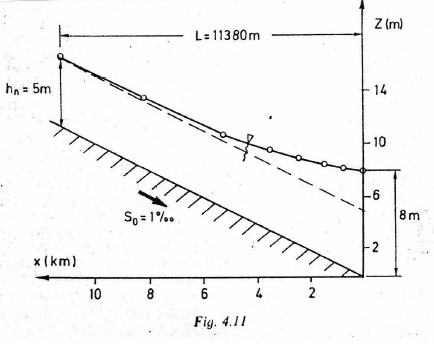
\includegraphics[width=5in]{./13-SteadyWSP/bw_curve1.jpg} 
   \caption{Example backwater curve} 
   \label{fig:example1}
\end{figure}
\newpage
\begin{lstlisting}[caption=R Console Output when script is run \\ , label=lst:backwaterConsole]
> # here is the function call
> backwater(begin_depth=8,end_depth=5,how_many=31,
    + discharge=55.4,width=5,mannings_n=0.02,slope=0.001)
         distance    depth        bse       wse
 [1,]      0.0000 8.000000  0.0000000  8.000000
 [2,]   -283.3504 7.806452  0.2833504  8.089802
 [3,]   -428.0112 7.709677  0.4280112  8.137689
 [4,]   -574.8516 7.612903  0.5748516  8.187755
 [5,]   -724.0433 7.516129  0.7240433  8.240172
 [6,]   -875.7785 7.419355  0.8757785  8.295133
... Many Rows ...
[29,]  -7186.0943 5.193548  7.1860943 12.379643
[30,]  -8389.5396 5.096774  8.3895396 13.486314
[31,] -11393.2010 5.000000 11.3932010 16.393201
\end{lstlisting} 

Figure \ref{fig:Rplot1} is the same situation computed and plotted using the script in this essay\footnote{With some additions that will be demonstrated in class!}.

\begin{figure}[h!] %  figure placement: here, top, bottom, or page
   \centering
   \includegraphics[width=5in]{./13-SteadyWSP/example1Rplot.pdf} 
   \caption{Backwater curve computed and plotted using \textbf{R}}
   \label{fig:Rplot1}
\end{figure}

~\newpage
\subsubsection{Example 2 --- Front-water curve}

Figure \ref{fig:example2} is another illustrative case.  Here the water discharges into a horizontal channel at a rate of $1 \frac{m^3}{sec}$ per meter width.  Assuming Manning's $n~\approx 0.01$ we wish to compute the profile downstream of the gate and determine if it will extend  to the sharp edge\footnote{Obviously the profile will change a lot near the edge, but the question is will the profile continue to rise as depicted if the edge were further away?}.

\begin{figure}[h!] %  figure placement: here, top, bottom, or page
   \centering
   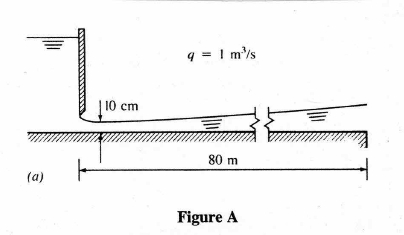
\includegraphics[width=4in]{./13-SteadyWSP/bw_curve2.jpg} 
   \caption{example caption}
   \label{fig:example2}
\end{figure}

We would need to know the critical depth for the section ($\approx 0.47 meters$), then compute the profile moving from the gate downstream (a frontwater curve with respect to the gate).  

With the \texttt{backwater} function, all we really need to do is change the function arguments because it is already built for rectangular channels.  

Observe that the distance is now incrementing forward (by choice of begin and end depths).  Figure \ref{fig:Rplot2} is the situation computed and plotted using the script.

\begin{lstlisting}[caption=R Console Output when script is run \\ , label=lst:frontwaterConsole]
> # The function --- note the changes in parameter values!
> backwater(begin_depth=0.1,end_depth=0.47,how_many=20,
   + discharge=1,width=1,mannings_n=0.01,slope=0.000)
      distance  depth bse    wse
 [1,]  0.00000 0.1000   0 0.1000
... Rows ...
[13,] 79.00486 0.3405   0 0.3405
[14,] 82.82243 0.3590   0 0.3590
... Rows ...
\end{lstlisting} 

\begin{figure}[h!] %  figure placement: here, top, bottom, or page
   \centering
   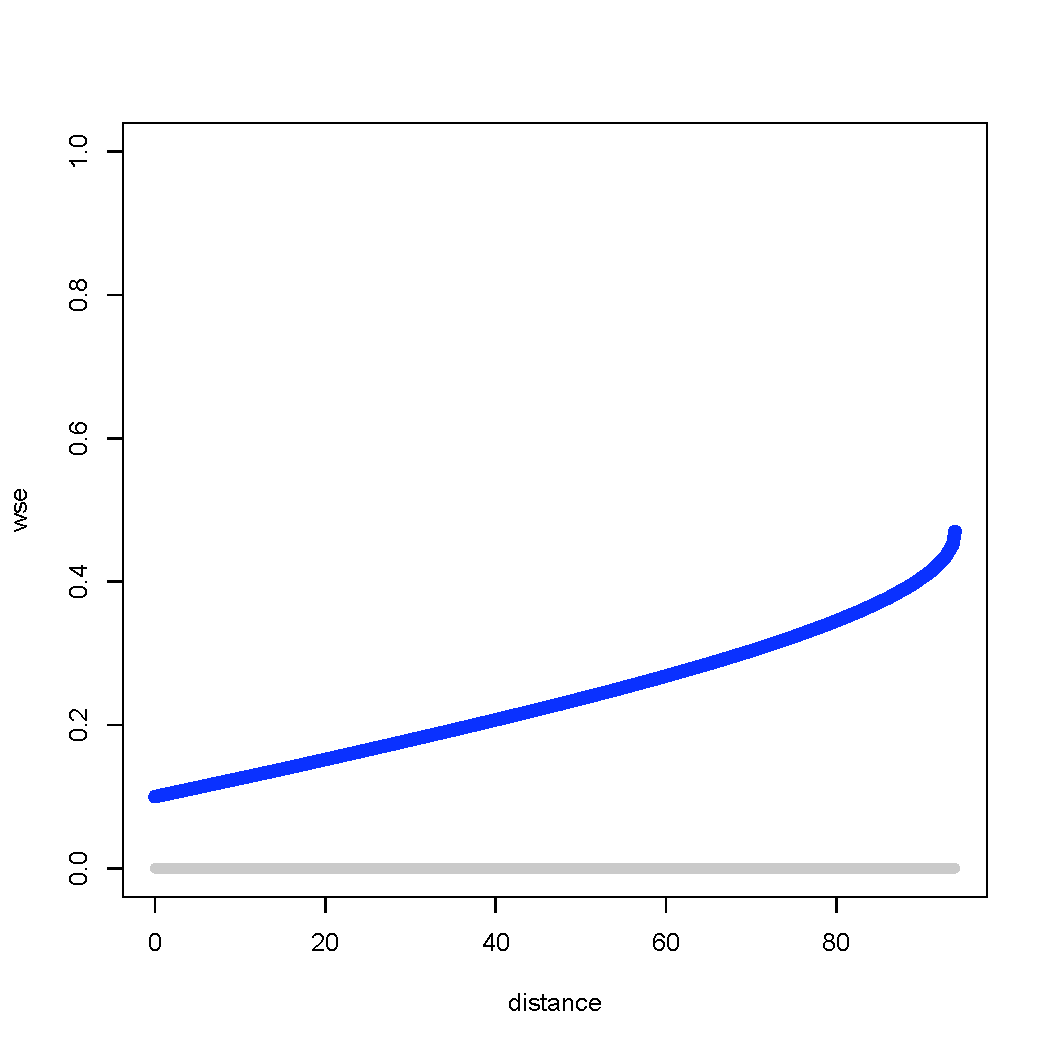
\includegraphics[width=4in]{./13-SteadyWSP/Example2Rplot.pdf} 
   \caption{Frontwater curve computed and plotted using \textbf{R}}
   \label{fig:Rplot2}
\end{figure}
\newpage
\subsubsection{Finite Difference Methods --- Fixed Space Change Method}
The fixed-depth change, variable-space result is a useful tool, but not terribly practical because we mostly perform engineering hydraulics calculations to estimate values (depth, pressure, force) at prescribed locations in space, so we need another approach to the problem where we can prescribe the spatial locations, and solve for the depths.

First the gradually varied flow equation is rearranged for relating the change in specific energy between two section to the spatial difference and the slope differences as
\begin{equation}
\Delta h_s = \Delta (h + \frac{V^2}{2g}) = \Delta x (S_o - S_f)
\label{eqn:gvf-energy-bal}
\end{equation}

The computation of $h_{i+1},V_{i+1}$ from $h_i,V_i$ is performed by iteration.
An initial value for $h_{i+1}$ that is known to be too large is used in Equation \ref{eqn:gvf-energy-bal} along with the known value of $h_i$ to compute a trial value $h_{s(i+1)}$.

Then the trial value is used in the right hand side of Equation \ref{eqn:gvf-energy-newl}
\begin{equation}
h_s = (h + \frac{V^2}{2g})
\label{eqn:gvf-energy-newl}
\end{equation}

The two trial values are compared and the next value of $h_{i+1}$ is computed by sucessively decreasing until the two values computed by the difference equation and the definition of specific energy coincide.  The example below uses a method from Hamming to make the comparisons and adjust the guesses until they are sufficiently close enough.

\textbf{Example (Non-Prismatic Channel), Fixed Spatial Steps)}\\
A plan view of a rectangular channel of variable width as shown in Figure \ref{fig:NonPrismaticExample}.
\begin{figure}[h!] %  figure placement: here, top, bottom, or page
   \centering
   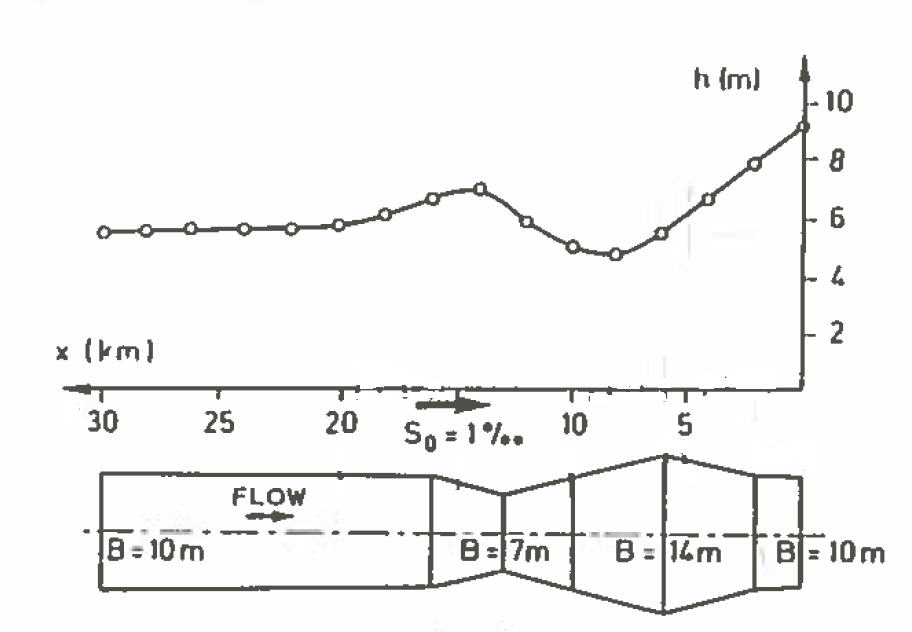
\includegraphics[width=3.4in]{./13-SteadyWSP/NonPrismaticExample} 
   \caption{Non-Prismatic Rectangular Channel}
   \label{fig:NonPrismaticExample}
\end{figure}
\newpage
The channel conveys $Q=100~m^3/sec$, with a bottom slope of $0.001$ and average Manning's $n$ value of $0.033$.  
A backwater curve is caused by a weir at the downstream end (to the right in the figure) by a 7 meter tall weir.
Flow depth over the weir is at critical depth $h_c = 2.17$ meters.  Normal flow in the upstream portion for 10-meter channel width is $h_n = 5.6$ meters.  Using the fixed space step method determine and plot a profile view of the water surface and channel bottom.

Figure \ref{fig:ExamplePlot} is a screen capture of the result for the example problem.  

\begin{figure}[h!] %  figure placement: here, top, bottom, or page
   \centering
   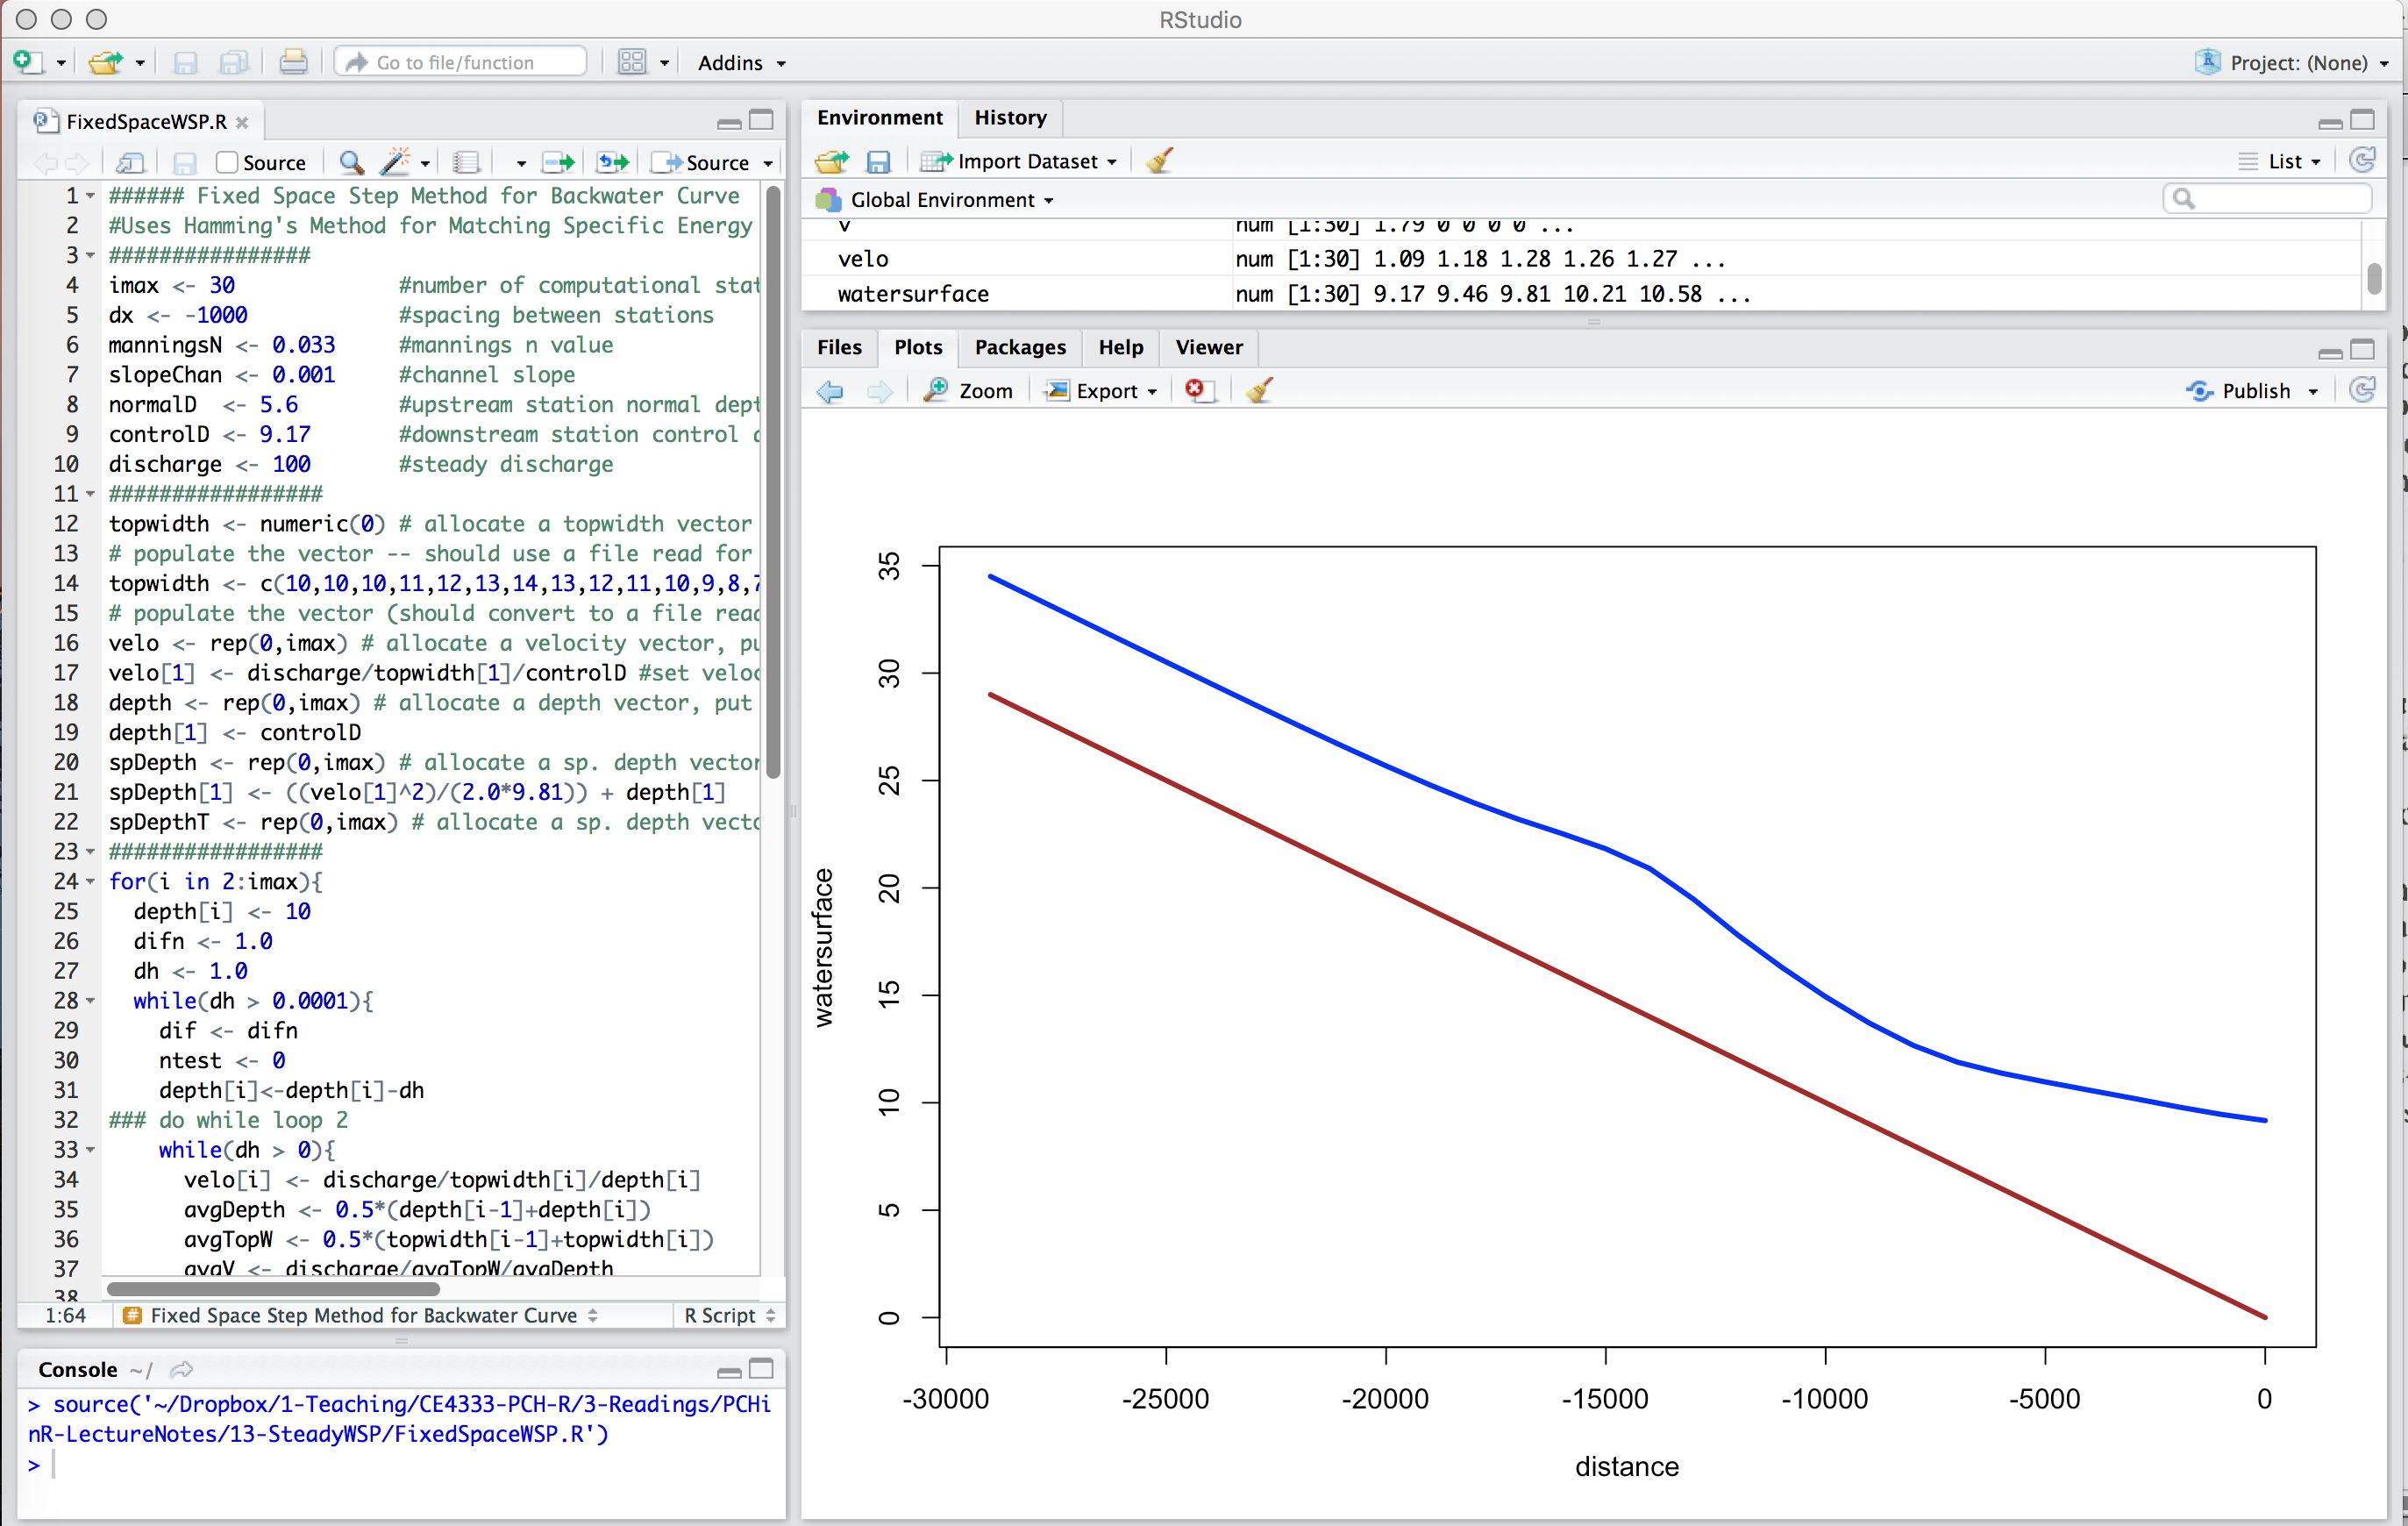
\includegraphics[width=5.6in]{./13-SteadyWSP/ExamplePlot.jpg} 
   \caption{Backwater curve computed and plotted using \textbf{R}}
   \label{fig:ExamplePlot}
\end{figure}

Listing \ref{lst:FixedSpaceMethod} is an entire listing for the example problem.  
The listing introduces our first intricate use of \texttt{for(...)}, \texttt{while(...)}, and the use of \texttt{break} to control the program logic.   The outer \texttt{for(...)} loop is used to step through the various cross sections while the two inner \texttt{while(...)} ``loops'' are used to perform the specific energy balancing logic and exit under different conditions.

In older languages where \texttt{goto ... <label>} was allowed logical control crossed over loopback paths.  
Computer scientists claimed that a  \texttt{goto ... <label>} was unnecessary -- this example here was ported from a \texttt{FORTRAN} code from the 1980's, and indeed the  \texttt{goto ... <label>} statements were not required.
\clearpage

\begin{lstlisting}[caption=R script for Backwater Curve by Fixed Space Method \\ , label=lst:FixedSpaceMethod]
###### Fixed Space Step Method for Backwater Curve  ###########
#Uses Hamming's Method for Matching Specific Energy at Sections
################
imax <- 30             #number of computational stations
dx <- -1000            #spacing between stations
manningsN <- 0.033     #mannings n value
slopeChan <- 0.001     #channel slope
normalD  <- 5.6        #upstream station normal depth
controlD <- 9.17       #downstream station control depth
discharge <- 100       #steady discharge
#################
topwidth <- numeric(0) # allocate a topwidth vector
# populate the vector -- should use a file read for general program
topwidth <- c(10,10,10,11,12,13,14,13,12,11,10,9,8,7,8,9,10,10,10,10,10,10,10,10,10,10,10,10,10,10)
# populate the vector (should convert to a file read)
velo <- rep(0,imax) # allocate a velocity vector, put zeroes everywhere
velo[1] <- discharge/topwidth[1]/controlD #set velocity at control section
depth <- rep(0,imax) # allocate a depth vector, put zeroes everywhere
depth[1] <- controlD
spDepth <- rep(0,imax) # allocate a sp. depth vector, put zeroes everywhere
spDepth[1] <- ((velo[1]^2)/(2.0*9.81)) + depth[1]
spDepthT <- rep(0,imax) # allocate a sp. depth vector, put zeroes everywhere
#################
for(i in 2:imax){
  depth[i] <- 10
  difn <- 1.0
  dh <- 1.0
  while(dh > 0.0001){
    dif <- difn
    ntest <- 0
    depth[i]<-depth[i]-dh
### do while loop 2
    while(dh > 0){
      velo[i] <- discharge/topwidth[i]/depth[i]
      avgDepth <- 0.5*(depth[i-1]+depth[i])
      avgTopW <- 0.5*(topwidth[i-1]+topwidth[i])
      avgV <- discharge/avgTopW/avgDepth
      hydR <- avgDepth*avgTopW/(avgTopW+2.0*avgDepth)
      sFric <- (avgV^2)*(manningsN^2)/(hydR^(1.33))
      spDepth[i] <- spDepth[i-1]+(slopeChan-sFric)*dx
      spDepthT[i] <- depth[i]+(velo[i]^2/(2.0*9.81))
      difn <- spDepthT[i]-spDepth[i]
 #     print(difn)
#      print(cbind(i,depth[i],spDepth[i],spDepthT[i],dh))
        if(ntest > 0){
          dh <- dh/10.0
          break #break from do while loop 2
          }
        if(dif*difn > 0){
          break #break from do while loop 2
        }
      depth[i] <- depth[i] + dh
      ntest <- 1
    } #do while loop 2
  } # do while loop 1
} # for loop
##### report results #####
# build x-vector
distance <- seq(0,(imax-1)*dx,dx)
bottom <- -distance*slopeChan
watersurface <- depth+bottom
plot(distance,watersurface,ylim=c(0,max(watersurface)),type="l",col="blue",lwd=3)
lines(distance,bottom,col="brown",lwd=3)
\end{lstlisting} 
%
%\subsection{Exercise Set 10}
%\begingroup
%\begin{center}
%{\textbf{{ CE 3305 Engineering Fluid Mechanics} \\ Exercise Set 23 \\ Summer 2018 -- GERMANY} }
%\end{center}
%\endgroup
%\begingroup
%~\newline
%\textbf{Purpose} : Apply computational hydraulics principles to compute steady water surface profiles in an open channel. \\
%\textbf{Assessment Criteria} : Completion, results plausible, format correct, \textbf{R} script shown\\~\\
%\textbf{Exercises}:
%\begin{enumerate}
%\item Modify the (variable space step method) \textbf{R} code for U.S. Customary units.  Use the modified function to compute the water surface profile for a wide rectangular channel with Manning's $n = 0.022$, bottom slope $S_0 = 0.0048$, and discharge per unit width of $\frac{Q}{W} = 5 \frac{ft^3}{sec}$.  Determine how far along the channel $x=L$ does it take for the flow depth to rise from a value of $y=3.0 ft$ to $y=4.0 ft$. Is the 4-ft depth position upstream or downstream of the 3-ft depth position?  Plot the water surface profile.\footnote{Guideline:  The profile should extend less than 400 feet for this problem --- if your profiles are going further, there is probably something wrong with your functions or input values.}.  
%\item Modify the (variable space step method) \texttt{area} and \texttt{perimeter} functions as well as the \texttt{backwater} functions for a trapezoidal channel.  Apply the modified functions for a trapezoidal channel with a [$2:1$] side slope, $3.5 ft$ bottom width, $0.012$ bed slope, that discharges from a reservoir at $Q=185 \frac{ft^3}{sec}$.  You should assume the upstream value is at critical depth ($\approx~2.7 ft$) and compute the profile to within $2\%$ of normal depth.  Plot the profile\footnote{Guideline:  The profile should extend less than 100 feet for this problem --- if your profiles are going further, there is probably something wrong with your functions or input values.} .
%\item Convert the fixed space step example problem into US customary units.  Then modify the script for US customary units and repeat the example. 
%\end{enumerate}

%These exercises are also located on the class server as \texttt{ES-10}




%%\subsection{References}
%Jaeger, C. (1957). Engineering Fluid Mechanics. St. Martin's Press. 529p. 
%
%Koutitas, C.G. (1983). Elements of Computational Hydraulics. Pentech Press, London 138p. ISBN 0-7273-0503-4 
